\section{The READEX Methodology} \label{sec:methodology}

The READEX methodology is split into two phases: design-time (during application development) and runtime (during production runs). READEX performs a sequence of steps to produce tuning advice for an application. The following sections describe the steps defined in the READEX methodology.

%\begin{figure}[!t]
%\centering
%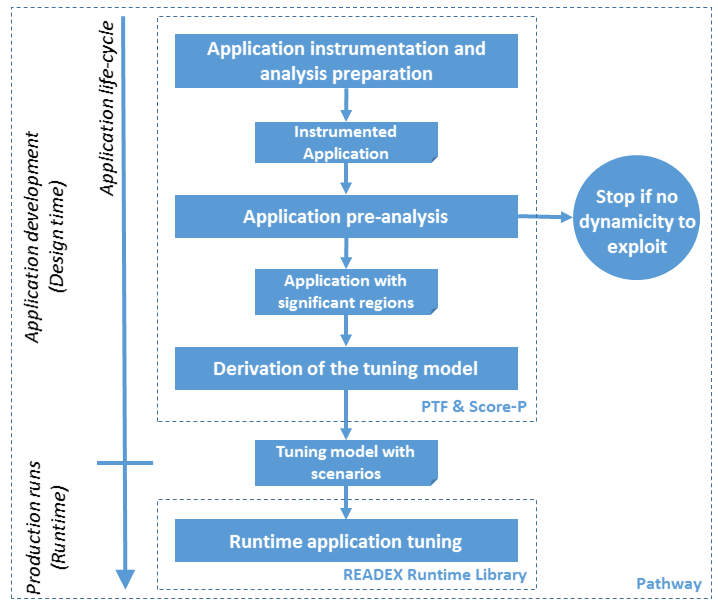
\includegraphics[width=.70\columnwidth]{figures/READEX_workflow.png}
%\caption{Overview of READEX methodology}
%\label{fig:readex_methodology}
%\end{figure}

\subsection{Application Instrumentation and Analysis Preparation}
\label{sec:application_instrumentation}
The first step in READEX is to instrument the HPC application by inserting probe-functions around different regions that are of interest to tuning. A region can be any arbitrary part of the code, for instance a function or a loop. READEX is based on instrumentation with Score-P and requires that the \textit{phase region} be manually annotated. A phase region is single-entry and exit region where most of the application progresses. Typically, a phase region may be the body of the main progress loop of the application. In addition to the phase region, READEX supports instrumentation of \textit{user regions} inside the phase region. User regions may be instrumented manually using Score-P or automatically by the compiler.

The READEX methodology also allows exposing parameters that define dynamic behaviour of the application. These parameters, referred to as additional identifiers, will enhance the distinction of different scenarios into runtime situations during the application execution, potentially leading to better identification of optimal configurations for the different tuning parameters. An example of additional identifiers is different input data sets. Exposing this information will allow READEX to detect different compute characteristics of the application caused by different inputs.

\subsection{Application Pre-analysis}
\label{sec:dynamism_detection}
After instrumenting an application and preparing it for analysis, the second step in the READEX approach is to perform a pre-analysis. The objective of this step is to automatically identify and characterise dynamism in the application behaviour. This is critical because the READEX approach is based on tuning hardware, system and application parameters based on the dynamism exhibited by the different regions in the application. READEX is capable of identifying and characterising two types of application dynamism:
\begin{itemize}
  \item \textit{Inter-phase dynamism}: This occurs when each phase (execution instance) of a phase region in the application exhibits different characteristics. This results in different values for the measured objective values (execution time) and thus may require different configurations to be applied for the tuning parameters.
  \item \textit{Intra-phase dynamism}: This occurs when each runtime situation (execution instance) of the significant regions in a phase region exhibits different characteristics and results in different values fo the measured objective values (execution time, compute intensity) and thus may need different configurations to be applied for the tuning parameters.
\end{itemize}
The pre-analysis also identifies the regions in the application that contribute significantly to the execution of an application and are referred to as \textit{significant regions}. If no dynamism is identified in the pre-analysis then the rest of the READEX steps should be aborted due to homogeneous behaviour of the application which will not yield any energy or performance savings from auto-tuning.

Listing \ref{lst:minimd_dynamism_summary} presents an example of the summary of significant regions and the dynamism identified by READEX in the miniMD application.

\lstset{language=[90]Fortran,
	basicstyle=\ttfamily\scriptsize,
	frame=tb,
	aboveskip=2mm,
	belowskip=2mm,
	showstringspaces=false,
	columns=flexible,
	breaklines=true,
	breakatwhitespace=true,
	keywordstyle=\color{black},
	commentstyle=\color{black},
	escapeinside={(@*}{*@)},
}
\begin{lstlisting}[caption={Summary of Application Pre-analysis},label=lst:minimd_dynamism_summary]
...
Significant regions are:

void Comm::borders(Atom&)
void ForceLJ::compute_halfneigh(Atom&, Neighbor&, int) [with int EVFLAG = 0; int GHOST_NEWTON = 1]
void ForceLJ::compute_halfneigh(Atom&, Neighbor&, int) [with int EVFLAG = 1; int GHOST_NEWTON = 1]
void Neighbor::build(Atom&)


Significant region information
==============================
Region name                  Min(t)          Max(t)       Time Dev.(%Reg) Ops/L3miss    Weight(%Phase)

void Comm::borders(Atom&)    0.001             0.001            2.6           109              0
void ForceLJ::compute_hal    0.013             0.014            2.9            97             68
void ForceLJ::compute_hal    0.016             0.016            0.0            91              1
void Neighbor::build(Atom    0.047             0.048            0.7           332             23


Phase information
=================
Min                  Max                  Mean                 Dev.(% Phase)        Dyn.(% Phase)

0.0138626            0.0664566            0.020337             72.731               258.612

...

SUMMARY:
========

Inter-phase dynamism due to variation of execution time of phases

No intra-phase dynamism due to time variation

Intra-phase dynamism due to variation in compute intensity of following significant regions

void ForceLJ::compute_halfneigh(Atom&, Neighbor&, int) [with int EVFLAG = 0; int GHOST_NEWTON = 1]
void Neighbor::build(Atom&)
\end{lstlisting}

\subsection{Derivation of Tuning Model}
\label{sec:tuning_model_generation}
\todo{reference relevant sections in the paper}

Following the identification of exploitable dynamism in the pre-analysis step, the third step is to explore the space of possible tuning configurations and identify the optimal configurations of the tuning parameters for the phases and runtime instances during the application execution. This analysis is performed by PTF (Periscope Tuning Framework) in conjunction with Score-P and RRL (READEX Runtime Library). PTF is allows for performing design-time analysis experiments through a number of possible search strategies (eg. exhaustive, individual and heuristic search based on generic algorithm) to identify the optimal configurations for the runtime instances of significant regions identified in the pre-analysis step that exhibit dynamism. To achieve this, Score-P provides the instrumentation and profiling platform, while the RRL provides the platform for libraries to tune hardware and system parameters. Additionally, READEX also has dedicated libraries that allow tuning application-specific parameters.

It is important to note that the additional identifiers specified during the instrumentation step are particularly key in providing additional domain knowledge to distinguish and identify different optimal configurations for runtime scenarios \cite{PACO17}.

After all scenarios are explored and optimal configurations are identified, the rts's are grouped into a limited number of scenarios, e.g. up to 20. Each scenario is associated with a common system configuration, and it is hence composed of rts's with identical or similar best configurations. The limitation in the number of scenarios inhibits a too frequent configuration switching at runtime that may result in higher overheads from auto-tuning. The set of scenarios, information about the rts's associated with the scenarios, and the optimal configurations for each scenario are stored by PTF in the form of a serialized text file called the Application Tuning Model (ATM), to be loaded and exploited during production runs at runtime.

\subsection{Runtime Application Tuning}
\label{sec:runtime_tuning}

Following the completion of DTA, production runs of the application can now be tuned at runtime using the optimal configurations summarized in the ATM using the RRL. The RRL monitors the application execution using the Score-P instrumentation, identifies the scenario that is encountered at runtime, and applies the corresponding optimal configurations for each scenario using the knowledge in the ATM to optimise the application's energy consumption. The RRL uses libraries that are loaded as plugins for setting different configurations for the parameters that are tuned by READEX.

\subsection{Pathway for READEX Workflow}
\label{sec:pathway_for_readex_workflow}

Since the READEX methodology has quite a number of steps, it uses Pathway to automate the entire workflow. Pathway \cite{Pathway:Petkov13} is a tool for designing and executing performance engineering workflows for HPC applications. Pathway provides an out-of-the box workflow template that can be configured to apply READEX on an application in a HPC system of choice. This way, Pathway can keep track of each step that must be completed in order to obtain the tuning results. Figure~\ref{fig:pathway_browser} presents an example of a custom browser in Pathway that summarizes the results from each step of applying READEX on the miniMD application. On the left, you see the tuned applications. On the right top you have a list of experiments with the READEX workflow. Below that are the results from the pre-analysis and then the ATM.

%\begin{figure}[!t]
%\centering
%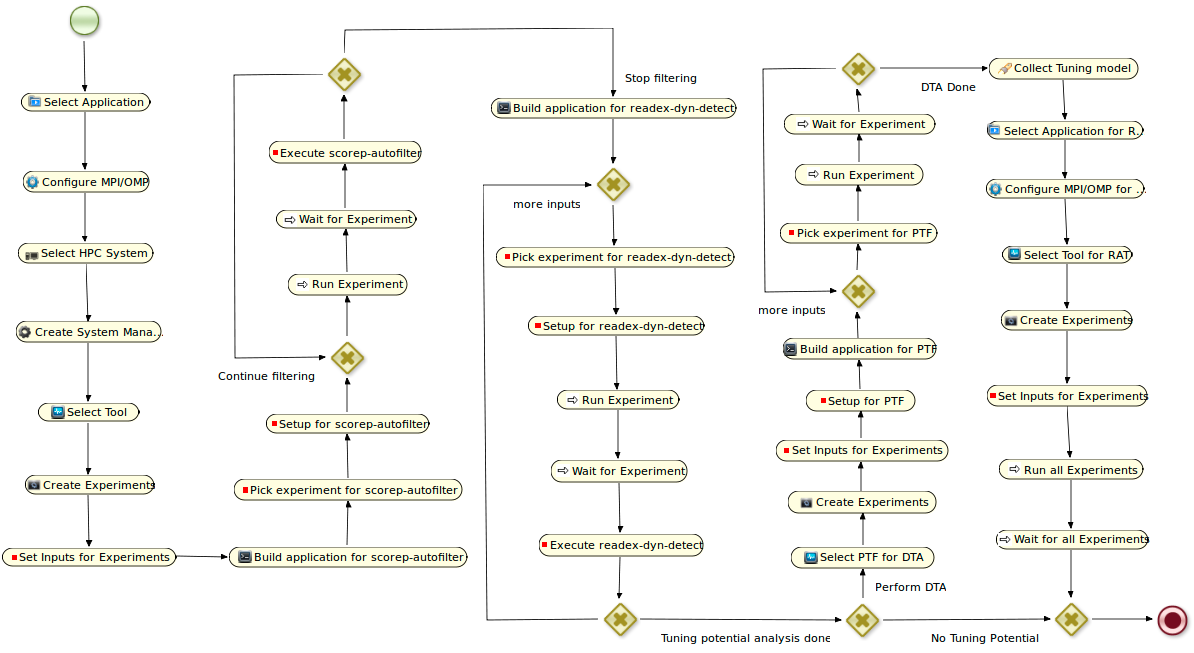
\includegraphics[width=.95\columnwidth]{figures/PathwayWorkflow.png}
%\caption{READEX Workflow in Pathway}
%\label{fig:pathway_workflow}
%\end{figure}

\begin{figure}[!t]
\centering
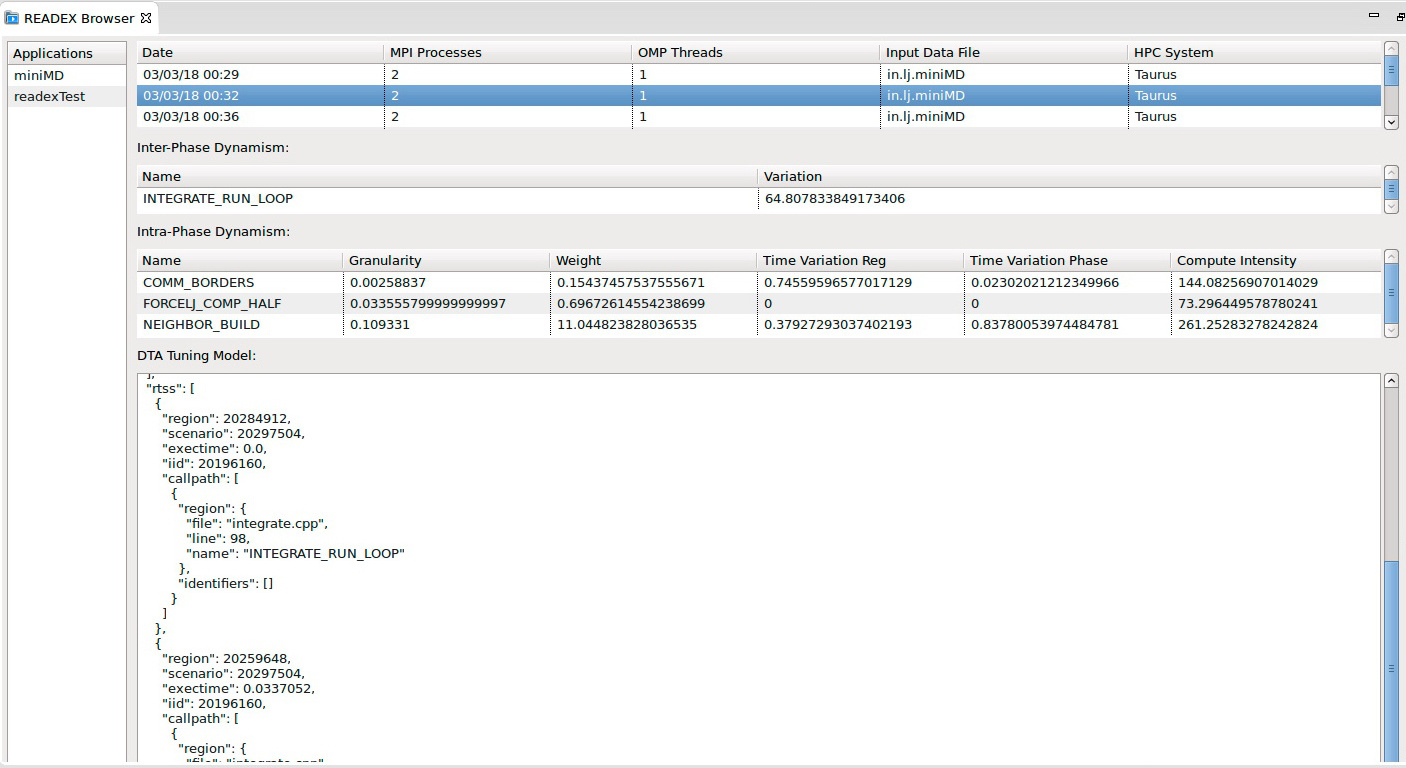
\includegraphics[width=.95\columnwidth]{figures/PathwayBrowser.jpeg}
\caption{READEX Results Browser in Pathway}
\label{fig:pathway_browser}
\end{figure}
